\section{Software Choice}
For the hardware components to interact, software parts are needed to handle them. The software choice is explained in this section, which describes the use of the chosen RTOS (Real Time Operating System), and the principle of scheduling.

\subsection{Real Time Operating System}
The chosen RTOS is a stable open source project named KRNL, written by the Associate Professor Jens Dalsgaard Nielsen from Aalborg University.\\
Specially written for the Arduino platform, it allows to control the tasks, and therefore the behaviour of the vehicle, through a timer, to keep a precise and constant time schedule. This property makes it possible to export it to another kind of processor and still have the same render, as long as it have a frequency high enough to process all the data needed.\\
One of KRNL's advantage is also the definition of semaphores, priorities, and critical regions, that the system will use to choose which task to run, and how often to run it. Futhermore, this RTOS allows to program in Arduino language, which is a C\texttt{++} extension, and can also run C code, using different files.

\subsection{Scheduling}\label{sec:scheduling}
To run the code on the Arduino microcontroller, and be able to manage all the sensors in parallel and at the time needed, a scheduling scheme is needed. Indeed, the microcontroller must be able to receive and process the data from the GoT computer received through the XBee module, the Hall sensors and the magnetometer. From all this data, it also has to make a decision regarding the planned route to follow. This decision must affect at the same time the speed of the motor, and the steering through the servo.
A description of the scheduling principle and its function will now be described.


\subsubsection{Semaphores}
In programming, a semaphore is a variable or abstract data that is used to prioritize the different tasks to use. It allows a multiprogramming, with functions that use different resources and time, and does not interact with each others directly. Running them independently ease the development of the code.


\subsubsection{Tasks}
The different functions of the vehicle have been separated into multiple tasks, that can switch regarding to their priority. Five tasks are created to control the vehicle:

\begin{lstlisting} [caption = {Implementation of the tasks}, label = {lst:tasks}]

  task1 = k_crt_task(tSpeed, 11, stack, 300);         	   // Hall Sensors
  task2 = k_crt_task(SpeedControl, 12, stack2, 300); 	   // Speed control
  task3 = k_crt_task(GoT,14,stack5,1000);        		   // GoT and protocol handling
  task4 = k_crt_task(LeadCompensator, 13, stack4, 300);    // Distance Control
  task5 = k_crt_task(SteeringControl, 10, stack3, 1000);   // Angular control

\end{lstlisting}

Those declarations of the tasks are made thanks to the function k\_crt\_task needing the name of the function to run, it's priority, the stack buffer to use and it's length. The implementation of this function can be seen below.


\begin{lstlisting} [caption = {Declaration of the tasks}, label = {lst:tasks}]
 struct k_t *k_crt_task (void (*pTask) (void), char prio, char *pStk, int stkSize);
 
\end{lstlisting}


\textbf{Hall Sensors:}
The two hall sensors of the two belts are read at a certain frequency, and knowing the distance the vehicle moves during a full turn of the drive wheel, the real speed of each belt can be calculated independently.\\
When the belts are not running the maximum time to run the task has been measured to \SI{5.63}{\mu s}, and when the belts are running it takes \SI{8.39}{\mu s}.
The maximum speed of vehicle is 3 $m \cdot s^{-1}$, and a turn of the gear wheel is 166mm. To get a pulse every full turn of the gear wheel at the highest speed, the sampling period has to be $\frac{\SI{0.166}{m\cdot s^{-1}}}{\SI{3}{m}}={\SI{55.3}{ms}}$, and for a quarter of turn it should be 4 time less so every 14ms. According to the Nyquist-Shannon Sampling Theoem, the sampling frequency of reading the hall sensors has to be at least 2 times higher than the highest frequency of the signal, but to be safe, the sampling frequency is chosen \SI{3.5}{} times higher, resulting in a sampling period of 4ms.

\textbf{Speed Control:}
A wanted speed value is compared to the actual speed, and the resulting error is the input of the Velocity PI-Controller, that will set a new duty cycle for the motor, according to the reference.\\
The running time of this task is 386µs. As the speed can only be regulated when new measurements has arrived from the hall sensors, there will be no real advantages to run this task faster than at a 14ms period, in a perfect world. But as this is a real system, a little margin is added, and the period is chosen as 10ms. 

\textbf{GoT System and Communication Protocol:}
This task is the communication protocol handling, that receives positions of the vehicle from the GoT system. It will receive data from the computer, and convert it into a distance from the perfect route, so that the distance control can calculate the new heading to follow.\\
The running time of the GoT System and Communication Protocol task is 395µs, and the sampling period of the GoT system is 100ms.

\textbf{Angular Control:}
The steering task gathers readings from the magnetometer, and transform them into the coordinate system that fits the model. Those values are then converted into a heading angle, that will be used in the steering P-Controller to calculate the new angle to send to the servo. This is the inner loop from the Steering Model, seen in \secref{sec:SteeringModel}.\\
The running time of the Angluar Control is the largest one with \SI{1.7}{ms} needed to process a new angle. However, the sampling time of the servo is 30ms, so it makes no sense to run the task more often than this. The period of this task is therefore chosen to be 30ms.\\

\textbf{Distance control:}
While the angular control is in charge of the direction of the vehicle, it can not control the parallel distance from the line wanted to be on. The task Distance Control calculate the distance of the vehicle from the line it should follow, and calculate a new heading for the angular control, to get back on the line. This is the outer loop from the Steering Model, seen in \secref{sec:SteeringModel}.\\
The running time of the Distance Control is \SI{153.6}{\mu s}. It only runs when the GoT System and Communication Protocol delivers new data, so this task will also run once every 100ms.

A recapitulation of the parameters can be seen on \tableref{scheduleParameters}.

\begin{table} [H]
	\begin{tabular}{|l|l|l|l|l|l|}
								
\hline
\textbf{n°}  & \textbf{Task}   	 & \textbf{Priority}	& \textbf{Max. Time to Run} 	& \textbf{Min. Period} & \textbf{CPU Used}\\
\hline
1			 &	Hall Sensors	 & 2				&	\si{8,39 \mu s}			    &	\si{4 ms}			  & 0,2\%	  \\
\hline
2			 &	Speed Control	 & 3				&	\si{386\ \mu s}				&	\si{10 ms}			  &	19,3 \%   \\
\hline
3			 &	GoT and Protocol & 4				&	\si{395 \mu s}			    &	\si{100 ms}			  &	0,395 \%  \\
\hline
4			 &	Distance Control & 4				&	\si{153,6 \mu s} 			&	\si{100 ms} 	  	  &	0,154 \%  \\
\hline
5			 &	Angular Control	 & 1				&	\si{1,7  ms}			    &	\si{30 ms}			  &	5,7 \%    \\
\hline		
	\end{tabular}
	\caption{Calculations of the steering parameters.}	
	\label{scheduleParameters}						
\end{table}	

In the \tableref{scheduleParameters}, the Maximum Time to Run is the time the task needs to complete a full turn of the loop. The Minimum Period is the sampling time for the task, to run every time period. The CPU used is the percentage used by the task of the CPU, which is the ratio between the Maximum Time to Run and the Minimum Period.

\subsubsection{Queue}
The tasks are meant to be executed at the time they are scheduled to, ensuring the good control of the vehicle. But some functionalities are not critical, and can wait until the processor have time to do them.\\
When a task is running and another one with a higher priority makes a request to run, the actual task will be paused and wait until the higher priority ones are done.

\subsubsection{Request and Priorities}
The tasks makes a request of to run every period of time according to their respective setup, the global view of these request can be seen in \figref{scheduleRequest}.

 \begin{figure}[H]
	\centering
	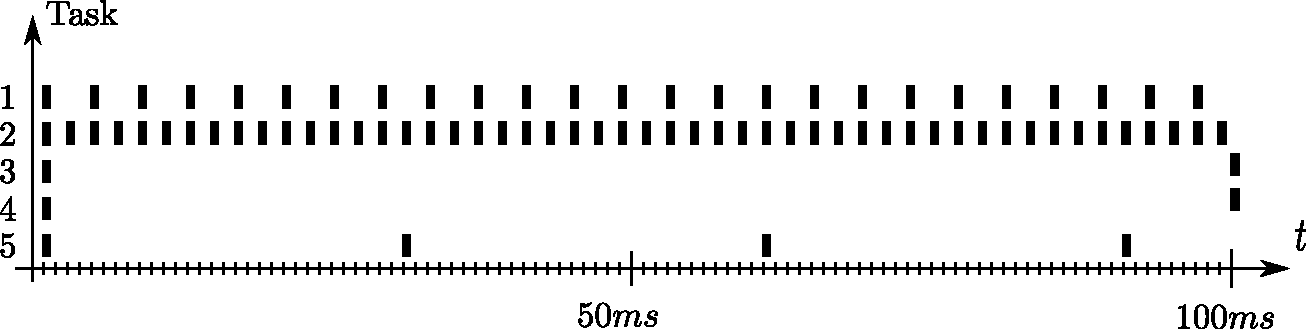
\includegraphics[scale=0.6]{figures/scheduleRequest.pdf}
	\caption{An overview of the tasks requests during 100ms.}
	\label{scheduleRequestd}
\end{figure}


When two task requests to run at the same time, the order is chosen according to the priorities, that are set at the initialisation. If the processor is free. the task are run when they ask for it, but interrupted when a higher priority task needs to run, and will finish when all the higher priority tasks are done. An example of this case can be seen in \figref{schedulePriorities}.\\
The priorities of the task have been made to give the system the best stability. In this case, The angular sensor has the highest priority because it has a large period and running time, but is critical to the steering of the vehicle which is the main objective of this project. Then comes the hall sensors that is very fast to execute, and then the speed control which is so fast that is not critical to have it at a high priority. The last one is the GoT system and communication protocol along with the distance control, because of two things: first because it may enter in an infinite loop and block the system if no data is received, and second and most of all because the main point of this project is to be able to run without the GoT system if something happens to block the communication.

 \begin{figure}[H]
	\centering
	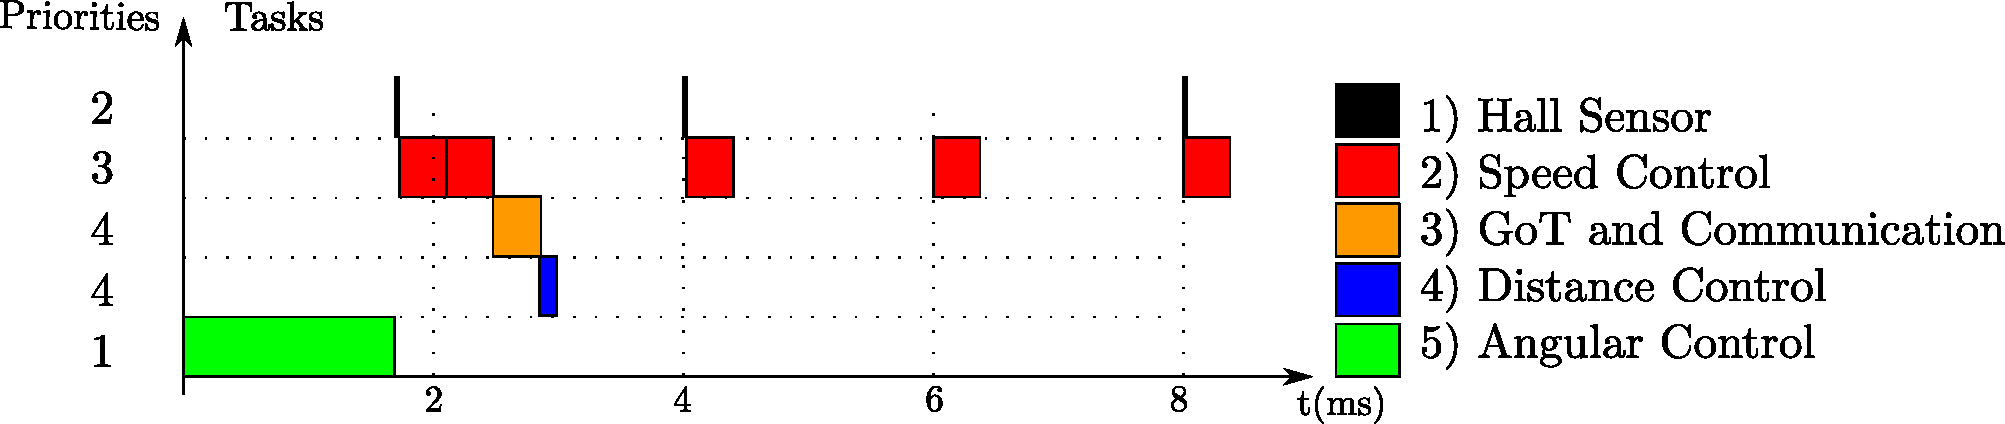
\includegraphics[scale=0.5]{figures/schedulePriorities.pdf}
	\caption{Schedule of the tasks at the starting time, regarding the priorities.}
	\label{schedulePriorities}
\end{figure}

As seen on the  \figref{schedulePriorities}, the angular control has the highest priority so it will run first, and the others will be registrered in a queue in order of priority. Then the hall sensors are second, and speed control after that. The GoT and comunication will run after them, and in the end the Distance Control.\\
After a certain time, the task running periods will stabilize, until the tasks with a large period are executed again.\\\\

Now that the hardware and software choices have been made, described and explained, the tasks for the sensors can be implemented, independently from each other.